\begin{dang}{Toán thực tế liên môn}	
\end{dang}
\subsubsection{Bài tập tự luận}
\begin{bt}%[1K1B4-6] 
	Nhiệt độ ngoài trời ở một thành phố vào các thời điểm khác nhau trong ngày có thể được mô phỏng bởi công thức	$$h(t)=29+ 3\sin\dfrac{\pi}{12}\left( t-9\right).$$ với $h$ tính bằng độ $C$ và $t$ là thời gian trong ngày tính bằng giờ.
	\begin{listEX}[2]
		\item Tính nhiệt độ lúc $ 12 $ giờ trưa.
		\item Tính thời gian nhiệt độ thấp nhất trong ngày.
	\end{listEX}
	\loigiai{
		\begin{listEX}[2]
			\item! Khi $ t=12 $ thì $ h(12)=29+3\sin\dfrac{\pi}{12}\left( 12-9\right)=29+3\sin\dfrac{\pi}{4}\approx 31{,}12 $.\\
			Vậy nhiệt độ lúc $ 12 $ giờ trưa khoảng $31{,}12$ độ $ C $.
			\item! Ta có 
			\begin{eqnarray*}
				& & -1\le\sin\dfrac{\pi}{12}\left( t-9\right)\le 1 \\
				&\Leftrightarrow & -3\le3\sin\dfrac{\pi}{12}\left( t-9\right)\le 3\\
				&\Leftrightarrow & 26\le29+3\sin\dfrac{\pi}{12}\left( t-9\right)\le 32.
			\end{eqnarray*}
			Do đó nhiệt độ thấp nhất trong ngày là $ 26 $ độ $ C $ khi $$\sin\dfrac{\pi}{12}\left( t-9\right)=-1\Leftrightarrow \dfrac{\pi}{12}\left( t-9\right)=-\dfrac{\pi}{2}+k2\pi \Leftrightarrow t=3+24k \quad (k\in \mathbb{Z}).$$
			Do $ 0\le t\le 24 $ nên $ k=0 $ suy ra $ t=3 $.\\
			Vậy lúc $ 3 $ giờ là thời gian nhiệt độ thấp nhất trong ngày.
		\end{listEX}
	}
\end{bt}


\begin{bt}%[1K1K4-6] 
	Số giờ có ánh sáng mặt trời của một thành phố A ở vĩ độ $40^\circ$ Bắc trong ngày thứ $t$ của một năm không nhuận được cho bởi hàm số
	$$d(t) = 3\sin \left[ \dfrac{\pi}{182} \cdot (t - 80)\right]  + 12 \text{ với }t\in \mathbb{Z} \text{ và } 0 \le t \le 365.$$
	Hỏi thành phố A có đúng $12$ giờ có ánh sáng mặt trời vào ngày nào trong năm?
	\loigiai{
		Thành phố A có đúng $12$ giờ có ánh sáng mặt trời nên 
		\begin{eqnarray*}
			& & 3\sin \left[ \dfrac{\pi}{182} \cdot (t - 80)\right]  + 12=12\\
			&\Leftrightarrow & \sin \left[ \dfrac{\pi}{182} \cdot (t - 80)\right]  =0\\
			&\Leftrightarrow& \dfrac{\pi}{182} \cdot (t - 80)=k\pi \Leftrightarrow t=80+182k.
		\end{eqnarray*}
		Vì $0 \le t \le 365\Leftarrow0 \le 80+182k \le 365 \Leftrightarrow -0{,}43\le k \le 1{,}57 $ vì $ k\in \mathbb{Z} $ nên $ k\in\{0;1\} $.\\
		Khi đó $ t=80 $ hoặc $ t=262 $.\\
		Vậy có hai ngày $ 80 $ và $ 262 $ thì thành phố A có đúng $ 12 $ giờ có ánh sáng mặt trời.}
\end{bt}


\begin{bt}%[1K1K4-6] 
	Giả sử một vật dao động điều hoa xung quanh vị trí cân bằng theo phương trình $$x=2\cos\left(5t-\dfrac{\pi}{6} \right) $$ Ở đây, thời gian $t$ tính bằng giây và quãng đường $x$ tính bằng centimét. Hãy cho biết trong khoảng thời gian từ $0$ đến $6$ giây, vật đi qua vị trí cân bằng bao nhiêu lần?
	\loigiai{
		Vật qua vị trí cân bằng khi $ x=0 $ khi đó ta có 
		\begin{eqnarray*}
			& &2\cos\left(5t-\dfrac{\pi}{6} \right)=0\\
			&\Leftrightarrow & 5t-\dfrac{\pi}{6}=\dfrac{\pi}{2}+{k\pi}\\
			&\Leftrightarrow & t=\dfrac{2\pi}{15}+\dfrac{k\pi}{5}.
		\end{eqnarray*}	
		Mà $ 0\le t\le 6\Leftrightarrow 0\le \dfrac{2\pi}{15}+\dfrac{k\pi}{5}\le 6\Leftrightarrow -0{,}67\le k\le 8{,}88 $.\\
		Vì $ k\in \mathbb{Z} $ nên $ k=\left\lbrace 0;1;2;3;4;5;6;7;8\right\rbrace  $.\\
		Vậy vật đi qua vị trí cân bằng $ 9 $ lần.
	}
\end{bt}







\begin{bt}%[1K1K4-6] 
	\immini{Một cây cầu có dạng cung $AB$ của đồ thị hàm số $y=4{,}2\cdot\cos\dfrac{x}{8}$ và được mô tả trong hệ trục toạ độ với đơn vị trục là mét như ở hình bên. Một sà lan chở khối hàng hoá được xếp thành hình hộp chữ nhật với độ cao $3$ m so với mực nước sông sao cho sà lan có thể đi qua được gầm cầu. Chứng minh rằng chiều rộng của khối hàng hoá đó phải nhỏ hơn $12{,}5$ m.}{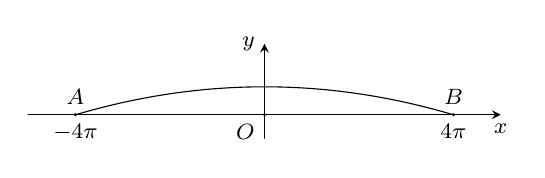
\begin{tikzpicture}[scale=0.6, font=\footnotesize, line join=round, line cap=round,>=stealth]
		\def\a{0} \def\b{-0.037} \def\c{0.59} % Hệ số
		\def\xmin{-5} \def\xmax{5}
		\def\ymin{-.5} \def\ymax{1.5}		
		\draw[->] (\xmin,0)--(\xmax,0) node [below]{$x$};
		\draw[->] (0,\ymin)--(0,\ymax) node [left]{$y$};
		\node at (0,0) [below left]{$O$};
		\fill (0,0)circle (1.0pt) (-4,0)node[above]{$A$} circle (1.0pt) (4,0)node[above]{$B$} circle (1.0pt) circle (1.0pt) (-4,0)node[below]{$-4\pi$} circle (1.0pt) (4,0)node[below]{$4\pi$} circle (1.0pt);
		\clip (-4,0) rectangle (4,1);
		\draw[smooth,samples=300] plot(\x,{\a*(\x)^4+\b*(\x)^2+\c});
		\end{tikzpicture}}
	\loigiai{
		Với mỗi điểm $ M $ nằm trên mặt cầu, khoảng cách từ điểm $ M $ đến mặt nước tương ứng với giá trị tung độ $ y $ của điểm $ M $,
		Xét phương trình $ 4{,}2\cdot \cos\dfrac{x}{8}=3\Leftrightarrow \cos \dfrac{x}{8}=\dfrac{5}{7}$.\\
		Do $ x\in [-4\pi;4\pi] $ nên $ \dfrac{x}{8}\in \left[-\dfrac{\pi}{2};\dfrac{\pi}{2} \right]  $.\\
		Khi đó, ta có $ \cos\dfrac{x}{8}=\dfrac{5}{7}\Leftrightarrow \dfrac{x}{8}\approx\pm 0{,}775 $, suy ra $ \left| \dfrac{x}{8}\right|<0{,}78\Leftrightarrow|x|<6{,}14$.\\
		Do sà lan có thể đi qua được gầm cầu nên chiều rộng của khối hàng hóa là $$ 2|x|<12{,}48<12{,}5. $$
	}
\end{bt}

\begin{bt}%[1K1K4-6] 
	Một quả đạn pháo được bắn ra khỏi nòng pháo với vận tốc ban đầu $ v_0=500$ m/s hợp với phương ngang một góc $ \alpha $. Trong Vật lí, ta biết rằng, nếu bỏ qua sức cản của không khí và coi quả đạn pháo được bắn ra từ mặt đất thi quỹ đạo của quả đạn tuân theo phương trình $ y=\dfrac{-g}{2v_0^2\cos^2\alpha}\cdot x^2+x\tan \alpha $, ở đó $g = 10$ m/s$ ^2 $ là gia tốc trọng trường.
	\begin{listEX}[2]
		\item! Tính theo góc bắn $\alpha$ tầm xa mà quả đạn đạt tới (tức là khoảng cách từ vị trí bắn đến điểm quả đạn chạm đất).
		\item!Tìm góc bắn $ \alpha $ để quả đạn trúng mục tiêu cách vị trí đặt khẩu pháo $22~000$ (m).
	\end{listEX}
	\loigiai{
		\begin{listEX}[2]
			\item! Ta có \begin{eqnarray*}
				y=0&\Leftrightarrow& \dfrac{-g}{2v_0^2\cos^2\alpha}\cdot x^2+x\tan \alpha=0\\
				&\Leftrightarrow & x\left(\dfrac{-g}{2v_0^2\cos^2\alpha}\cdot x+\tan \alpha \right)=0 \\
				&\Leftrightarrow & \hoac{&x=0\\&x=\dfrac{v_0^2\sin2\alpha}{g}= 25~000\sin2\alpha.}
			\end{eqnarray*}
			Vậy tầm bay xa mà quả đạn đạt tới là $25~000\sin2\alpha$ (m).
			\item! Điều kiện $ 0\le\alpha\le \dfrac{\pi}{2}$\\Để quả đạn trúng mục tiêu cách vị trí đặt khẩu pháo $22~000$ (m) thì
			\begin{eqnarray*}
				25~000\sin2\alpha =22~000	& \Leftrightarrow & \sin 2\alpha =\dfrac{22}{25}\\
				&\Rightarrow & 2\alpha\approx 1{,}08 \Leftrightarrow \alpha \approx 0{,}54.	\end{eqnarray*}
			Vậy góc bắn khoảng $ 0{,}54 \text{ (rad) }\approx 30{,}82^\circ $ thì quả đạn trúng mục tiêu cách vị trí đặt khẩu pháo $22~000$ (m).
	\end{listEX}	}
\end{bt}
\subsubsection{Bài tập trắc nghiệm}
\Opensolutionfile{ans}[ans/ans-1K1-4-Dang6]
\begin{ex}%[1K1Y4-6] 
	Nhiệt độ ngoài trời ở một thành phố vào các thời điểm khác nhau trong ngày có thể được mô phỏng bởi công thức	$h(t)=30+ 3\sin\dfrac{\pi}{12}\left( t-5\right)$. Với $h$ tính bằng độ $C$ và $t$ là thời gian trong ngày tính bằng giờ. Nhiệt độ lúc $ 7 $ giờ sáng là bao nhiêu?
	\choice
	{\True $31{,}5$ độ $ C $}
	{$32{,}5$ độ $ C $}
	{$30$ độ $ C $}
	{$37$ độ $ C $}	
	\loigiai{
		Khi $ t=7 $ thì $ h(7)=30+3\sin\dfrac{\pi}{12}\left( 7-5\right)=30+3\sin\dfrac{\pi}{6}= 31{,}5 $.\\
		Vậy nhiệt độ lúc $ 7 $ giờ trưa là $31{,}5$ độ $ C $.
	}
\end{ex}


\begin{ex}%[1K1B4-6] 
	Nhiệt độ ngoài trời ở một thành phố vào các thời điểm khác nhau trong ngày có thể được mô phỏng bởi công thức	$$h(t)=29+ 3\sin\dfrac{\pi}{12}\left( t-9\right).$$ với $h$ tính bằng độ $C$ và $t$ là thời gian trong ngày tính bằng giờ. Thời gian nhiệt độ cao nhất trong ngày là
	\choice
	{$ 13 $ giờ}
	{\True $ 15 $ giờ}
	{$ 12 $ giờ}
	{$ 14 $ giờ}
	\loigiai{Ta có 
		\begin{eqnarray*}
			& & -1\le\sin\dfrac{\pi}{12}\left( t-9\right)\le 1 \\
			&\Leftrightarrow & -3\le3\sin\dfrac{\pi}{12}\left( t-9\right)\le 3\\
			&\Leftrightarrow & 26\le29+3\sin\dfrac{\pi}{12}\left( t-9\right)\le 32.
		\end{eqnarray*}
		Do đó nhiệt độ cao nhất trong ngày là $ 32 $ độ $ C $ khi $$\sin\dfrac{\pi}{12}\left( t-9\right)=1\Leftrightarrow \dfrac{\pi}{12}\left( t-9\right)=\dfrac{\pi}{2}+k2\pi \Leftrightarrow t=15+24k \quad (k\in \mathbb{Z}).$$
		Do $ 0\le t\le 24 $ nên $ k=0 $ suy ra $ t=15 $.\\
		Vậy lúc $ 15 $ giờ là thời gian nhiệt độ cao nhất trong ngày.
	}
\end{ex}

\begin{ex}%[1K1Y4-6] 
	Số giờ có ánh sáng mặt trời của một thành phố A trong ngày thứ $t$ của một năm không nhuận được cho bởi hàm số
	$d(t) = 4\sin \left[ \dfrac{\pi}{18} \cdot (t - 80)\right]  + 12 \text{ với }t\in \mathbb{Z} \text{ và } 0 \le t \le 365$. Số giờ nắng của ngày thứ $ 83 $ là
	\choice
	{$ 12 $}
	{$ 11 $}
	{\True $ 14 $}
	{$8 $}
	\loigiai{
		Với $ t=83 $ thì $ d(83)=4\sin \left[ \dfrac{\pi}{18} \cdot (83 - 80)\right]  + 12=14 $.
		Vậy ngày thứ $ 83 $ có $ 14 $ giời nắng.
	}
\end{ex}

\begin{ex}%[1K1K4-6] 
	Số giờ có ánh sáng mặt trời của một thành phố $A$ trong ngày thứ $t$ trong một năm không nhuận được cho bởi công thức $$d(t) = 4\sin \left[\dfrac{\pi}{182}\left(t - 70\right) \right] + 16 \text{ với } t \in \mathbb{R} \text{ và } 0 < t \le 365.$$ Vào ngày nào trong năm thì thành phố $A$ có ít ánh sáng mặt trời nhất
	\choice
	{$353$}
	{$171$}
	{$161$}
	{\True $343$}
	\loigiai{
		Ta có $12 = 16 - 4 \le 4\sin \left[\dfrac{\pi}{182}\left(t - 70\right) \right] + 16 \le 16 + 4 = 20$.\\
		Do đó ngày có ít ánh nắng mặt trời nhất khi
		\begin{eqnarray*}
			dt = 12	& \Leftrightarrow & 4\sin \left[\dfrac{\pi}{182}\left(t - 70\right) \right] + 16 = 12 \Leftrightarrow \sin \left[\dfrac{\pi}{182}\left(t - 70\right) \right] = - 1\\
			&\Leftrightarrow & \dfrac{\pi}{182}\left(t - 70\right) = - \dfrac{\pi}{2} + k2\pi \Leftrightarrow t = - 21 + 364k \Rightarrow t = 343.
	\end{eqnarray*} }
\end{ex}

\begin{ex}%[1K1K4-6] 
	Hằng ngày mực nước con kênh lên xuống theo thủy triều. Độ sâu $ h$ (mét) của mực nước trong kênh được tính tại thời điểm $ t$ (giờ) trong một ngày bởi công thức $ h=3\cos\left(\dfrac{\pi t}{8}+\dfrac{\pi}{4}\right)+12$. Mực nước của kênh cao nhất khi $ t=t_0$. Tính giá trị của $ P=t_0^2+t_0$.
	\choice
	{$ t=272$}
	{$ t=182$}
	{$ t=240$}
	{\True $ t=210$}
	\loigiai{
		Mực nước cao nhất của kênh đạt được khi
		\begin{align*}
		\cos \left(\frac{\pi t_0}{8}+\frac{\pi}{4}\right)=1 \Leftrightarrow \frac{\pi t_0}{8}+\frac{\pi}{4}= k2\pi, k\in\mathbb{Z} \Leftrightarrow t_0=16k -2, k\in \mathbb{Z}.
		\end{align*} 
		Do $0\le t_0\le 24$ nên $k=1$ và $t_0=14$. Vậy $P=210$.
	}
\end{ex}

\begin{ex}%[1K1K4-6] 
	Số giờ có ánh sáng của thành phố Hà Nội trong ngày thứ $t$ của năm $2019$ được cho bởi một hàm số $y=4 \sin \left|\dfrac{\pi}{178}(t-60)\right|+10$, với $t\in\mathbb{Z}$ và $0<t\leq 365$. Vào ngày nào trong năm thì thành phố có ít giờ ánh sáng mặt trời nhất?
	\choice
	{\True $23$ tháng $11$}
	{$24$ tháng $11$}
	{$25$ tháng $11$}
	{$22$ tháng $11$}
	\loigiai{
		Do $\sin x\geq -1$  nên số giờ thành phố Hà Nội có ít ánh sáng mặt trời nhất  
		$\sin \left|\dfrac{\pi}{178}(t-60)\right|\geq -1$ với $t\in\mathbb{Z}$ và $0<t \leq 365$
		\begin{eqnarray*}
			&\Leftrightarrow& \left|\dfrac{\pi}{178}(t-60)\right|=\dfrac{3\pi}{2}+k2\pi\\
			&\Leftrightarrow&\hoac{&  \heva{& 60\leq t\leq 365 \\ &\dfrac{\pi}{178}(t-60)= \dfrac{3\pi}{2}+k2\pi} \\ & \heva{& 0< t\leq 60 \\ &\dfrac{\pi}{178}(60-t)= \dfrac{3\pi}{2}+k2\pi}}\\
			&\Leftrightarrow&\hoac{&  \heva{& 60\leq t\leq 365 \\ &t=327+k356}\\ & \heva{& 0< t<60 \\ &t=-207-k356}}\\
			&\Leftrightarrow& t=327\;(\text{vì }k\in\mathbb{Z}).
		\end{eqnarray*}
		Vậy thành phố Hà Nội có ít giờ ánh sáng nhất trong năm là ngày thứ $327$ của năm, tức là ngày $23$ tháng $11$ ($=365-31-7$).
	}
\end{ex}



\begin{ex}%[1K1K4-6] 
	Hằng ngày mực nước con kênh lên xuống theo thủy triều. Độ sâu $ h$ (mét) của mực nước trong kênh được tính tại thời điểm $ t$ (giờ) trong một ngày bởi công thức $ h=3\cos\left(\dfrac{\pi t}{8}+\dfrac{\pi}{4}\right)+12$. Mực nước của kênh cao nhất khi $ t=t_0$. Tính giá trị của $ P=t_0^2+t_0$.
	\choice
	{$ t=272$}
	{$ t=182$}
	{$ t=240$}
	{\True $ t=210$}
	\loigiai{
		Mực nước cao nhất của kênh đạt được khi
		\begin{align*}
		\cos \left(\frac{\pi t_0}{8}+\frac{\pi}{4}\right)=1 \Leftrightarrow \frac{\pi t_0}{8}+\frac{\pi}{4}= k2\pi, k\in\mathbb{Z} \Leftrightarrow t_0=16k -2, k\in \mathbb{Z}.
		\end{align*} 
		Do $0\le t_0\le 24$ nên $k=1$ và $t_0=14$. Vậy $P=210$.
	}
\end{ex}

\begin{ex}%[1K1K4-6] 
	Hằng ngày mực nước của con kênh lên, xuống theo thủy triều. Độ sâu $h$ (m) của mực nước trong kênh được tính tại thời điểm $t$ (giờ), $0\le t\le 24$ trong một ngày được tính bởi công thức $h(t)=3\cos \left(\dfrac{\pi t}{8}+\dfrac{\pi}{4} \right)+3$. Hỏi trong một ngày có mấy thời điểm mực nước của con kênh đạt độ sâu lớn nhất?
	\choice
	{ \True $1$}
	{ $3$}
	{ $2$}
	{ $4$}
	\loigiai{
		Thời điểm mực nước của con kênh đạt độ sâu lớn nhất khi và chỉ khi$$\cos \left(\dfrac{\pi t}{8}+\dfrac{\pi}{4} \right)=1\Leftrightarrow \dfrac{\pi t}{8}+\dfrac{\pi}{4}=k2\pi \Leftrightarrow t=-2+k16.$$
		Vì $0\le t\le 24$ nên $0\le -2+k16\le 24\Leftrightarrow \dfrac{1}{8}\le k\le \dfrac{13}{6}\Rightarrow k=1,k\in \mathbb{Z}$.}
\end{ex}


\begin{ex}%[1K1K4-6] 
	Giả sử một vật dao động điều hoa xung quanh vị trí cân bằng theo phương trình $x=2\sin\left(5t-\dfrac{\pi}{6} \right) $. Ở đây, thời gian $t$ tính bằng giây và quãng đường $x$ tinh bằng centimét. Vật đi qua vị trí cân bằng bao nhiêu lần trong $ 3 $ giây đầu.
	\choice
	{\True $ 5 $}
	{$ 3 $}
	{$ 4 $}
	{$ 8 $}
	\loigiai{
		Vật qua vị trí cân bằng khi $ x=0 $ khi đó ta có 
		\begin{eqnarray*}
			& &2\sin\left(5t-\dfrac{\pi}{6} \right)=0\\
			&\Leftrightarrow & 5t-\dfrac{\pi}{6}={k\pi}\\
			&\Leftrightarrow & t=\dfrac{\pi}{30}+\dfrac{k\pi}{5}.
		\end{eqnarray*}	
		Mà $ 0\le t\le 3\Leftrightarrow 0\le \dfrac{\pi}{30}+\dfrac{k\pi}{5}\le 3\Leftrightarrow -0{,}17\le k\le 4{,}61 $.\\
		Vì $ k\in \mathbb{Z} $ nên $ k=\left\lbrace 0;1;2;3;4\right\rbrace  $.\\
		Vậy vật đi qua vị trí cân bằng $ 5 $ lần.
	}
\end{ex}

\begin{ex}%[1K1K4-6] 
	Một quả đạn pháo được bắn ra khỏi nòng pháo với vận tốc ban đầu $ v_0=500$ m/s hợp với phương ngang một góc $ \alpha $. Trong Vật lí, ta biết rằng, nếu bỏ qua sức cản của không khí và coi quả đạn pháo được bắn ra từ mặt đất thi quỹ đạo của quả đạn tuân theo phương trình $ y=\dfrac{-g}{2v_0^2\cos^2\alpha}\cdot x^2+x\tan \alpha $, ở đó $g = 10$ m/s$ ^2 $ là gia tốc trọng trường. Góc bắn $ \alpha $ để quả đạn bay xa nhất là
	\loigiai{
		Ta có \begin{eqnarray*}
			y=0&\Leftrightarrow& \dfrac{-g}{2v_0^2\cos^2\alpha}\cdot x^2+x\tan \alpha=0\\
			&\Leftrightarrow & x\left(\dfrac{-g}{2v_0^2\cos^2\alpha}\cdot x+\tan \alpha \right)=0 \\
			&\Leftrightarrow & \hoac{&x=0\\&x=\dfrac{v_0^2\sin2\alpha}{g}= 25~000\sin2\alpha.}
		\end{eqnarray*}
		Vậy tầm bay xa mà quả đạn đạt tới là $25~000\sin2\alpha$ m.\\
		Vậy đạn bay xa nhất khi $ \sin2\alpha=1\Leftrightarrow 2\alpha=\dfrac{\pi}{2}+k2\pi\Leftrightarrow \alpha =\dfrac{\pi}{4}+k\pi $.\\
		Vì $ 0\le\alpha\le \dfrac{\pi}{2} $ nên $ \alpha=\dfrac{\pi}{4} $.\\
		Vậy góc bắn bằng $ 45^\circ $ thì đạn bay xa nhất.
	}
\end{ex}


